\documentclass{article}
\usepackage{mathtools}
\usepackage{amsmath, amssymb}
\usepackage{graphicx}
\begin{document}
\section*{Problem Statement}
The sum of the squares of the first ten natural numbers is,
\begin{gather*}
	1^{2} + 2^{2}+ ... + 10 = 385
\end{gather*}
The square of the sum of the first ten natural numbers is,
\begin{gather*}
	(1 + 2 + ... + 10)^{2} = 55^{2} = 3025
\end{gather*}
Hence the difference between the sum of the squares of the first ten natural numbers and the square of the sum is $3025 - 385 = 2640$.\\[12pt]

\noindent Find the difference between the sum of the squares of the first one hundred natural numbers and the square of the sum.
\section*{Solution}
Much like with the first problem, this problem is trivial to solve with a computer without using any fancy formulas. However, it can be broken down through sum formulas:
\begin{gather*}
	\sum_{i = 1}^{n}i = \frac{n(n + 1)}{2}\\
	\sum_{i = 1}^{n}i^{2} = \frac{n(n + 1)(2n + 1)}{6}
\end{gather*}
So:
\begin{gather*}
\left(\sum_{i = 1}^{n}i\right)^{2} - \sum_{i = 1}^{n}i^{2} = \left(\frac{n(n+1)}{2}\right)^{2} -  \frac{n(n + 1)(2n + 1)}{6}
\end{gather*}
A proof of the first formula can be found my first Project Euler solution. A derivation of the second formula can be found below. Simplifying:
\begin{align*}
	\left(\sum_{i = 1}^{n}i\right)^{2} - \sum_{i = 1}^{n}i^{2} &= \frac{n^{2}(n+1)^{2}}{4} -  \frac{n(n + 1)(2n + 1)}{6}\\
	&= n(n + 1)\left(\frac{3n(n + 1) - 2(2n + 1)}{12}\right)\\
	&= n(n + 1)\left(\frac{3n^{2} - n - 2}{12}\right)
\end{align*}
Checking:
\begin{gather*}
	n = \implies 10(11)(288)/12 = 2640
\end{gather*}
Plugging in:
\begin{gather*}
	n = 100 \implies 100(101)(29898)/12 = 25,164,150
\end{gather*}
which is confirmed by the algorithm.
\section*{Deriving Sum Formulas}
Based on the proof of the sum formula for $i$, once a formula has been found for the sum, proving that it is the sum is a matter of properly apply proof by induction. However, the real work of the problem is coming up with a proper formula. Thus consider the values of the sum:
\begin{align*}
n &\quad \sum_{i = 1}^{n}i^{2}\\
1 &\quad 1\\
2 &\quad 5\\
3 &\quad 14\\
4 &\quad 30\\
5 &\quad 55\\
6 &\quad 91\\
7 &\quad 140
\end{align*}
plotted below.
\newpage
\begin{figure}
	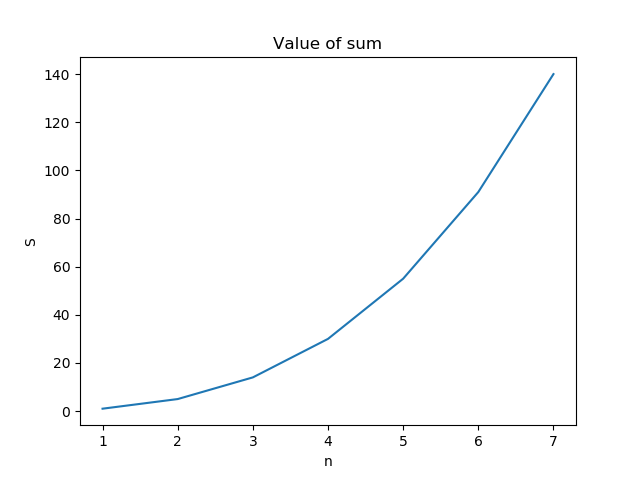
\includegraphics{Figure_1.png}
\end{figure}
It would be nice if, like the first sum formula, this formula was also a polynomial in terms of $n$. Based on the values, I will first attempt to fit it to a parabola:
\begin{gather*}
	S = an^{2} + bn + c
\end{gather*}
which gives the following linear system:
\begin{gather*}
	\begin{bmatrix}
		1 & 1 & 1\\
		4 & 2 & 1\\
		9 & 3 & 1
	\end{bmatrix}
	\begin{bmatrix}
		a\\
		b\\
		c
	\end{bmatrix}
	=
	\begin{bmatrix}
		1\\
		5\\
		14
	\end{bmatrix}
\end{gather*}
Putting in lower echelon form:
\begin{gather*}
	\begin{bmatrix}
		1 & 1 & 1\\
		4 & 2 & 1\\
		9 & 3 & 1
	\end{bmatrix}
	\begin{bmatrix}
		1\\
		5\\
		14
	\end{bmatrix} \rightarrow	
	\begin{bmatrix}
		1 & 1 & 1\\
		4 & 2 & 1\\
		0 & -2 & -2
	\end{bmatrix}
	\begin{bmatrix}
		1\\
		5\\
		3
	\end{bmatrix} \rightarrow	
	\begin{bmatrix}
		1 & 1 & 1\\
		0 & -2 & -3\\
		0 & -2 & -2
	\end{bmatrix}
	\begin{bmatrix}
		1\\
		1\\
		3
	\end{bmatrix} \rightarrow	
	\begin{bmatrix}
		1 & 1 & 1\\
		0 & -2 & -3\\
		0 & 0 & 1
	\end{bmatrix}
	\begin{bmatrix}
		1\\
		1\\
		2
	\end{bmatrix}	
\end{gather*}
So $c = 2$ and:
\begin{gather*}
	-2b - 6 = 1 \implies b = -7/2\\
	a - 7/2 + 2 = 1 \implies a = 5/2
\end{gather*}
Verifying the solution:
\begin{gather*}
	(5/2) - 7/2 + 2 = 1\\
	(5/2)(4) - (7/2)(2) + 2 = 5\\
	(5/2)(9) - (7/2)(3) + 2 = 14\\
	(5/2)(16) - (7/2)(4) + 2 = 28
\end{gather*}
which is not correct for $n = 4$. Thus, a parabola is an insufficient polynomial. Let's try then a cubic polynomial, repeating the process:
\begin{gather*}
	S = an^{3} + bn^{2} + cn + d
\end{gather*}
\begin{gather*}
	\begin{bmatrix}
		1 & 1 & 1 & 1\\
		8 & 4 & 2 & 1\\
		27 & 9 & 3 & 1\\
		64 & 16 & 4 & 1
	\end{bmatrix}
	\begin{bmatrix}
		a\\
		b\\
		c\\
		d
	\end{bmatrix}
	=
	\begin{bmatrix}
		1\\
		5\\
		14\\
		30
	\end{bmatrix}
\end{gather*}
Solving, by once again:
\begin{gather*}
	\begin{bmatrix}
		1 & 1 & 1 & 1\\
		8 & 4 & 2 & 1\\
		27 & 9 & 3 & 1\\
		64 & 16 & 4 & 1
	\end{bmatrix}
	\begin{bmatrix}
		1\\
		5\\
		14\\
		30
	\end{bmatrix} \rightarrow
	\begin{bmatrix}
		1 & 1 & 1 & 1\\
		8 & 4 & 2 & 1\\
		27 & 9 & 3 & 1\\
		0 & -8 & -6 & -4 
	\end{bmatrix}
	\begin{bmatrix}
		1\\
		5\\
		14\\
		-5
	\end{bmatrix} \rightarrow
	\begin{bmatrix}
		1 & 1 & 1 & 1\\
		8 & 4 & 2 & 1\\
		0 & -6 & -6 & -5\\
		0 & -8 & -6 & -4 
	\end{bmatrix}
	\begin{bmatrix}
		1\\
		5\\
		-4\\
		-5
	\end{bmatrix}\\
	\begin{bmatrix}
		1 & 1 & 1 & 1\\
		0 & -4 & -6 & -7\\
		0 & -6 & -6 & -5\\
		0 & -8 & -6 & -4 
	\end{bmatrix}
	\begin{bmatrix}
		1\\
		-3\\
		-4\\
		-5
	\end{bmatrix} \rightarrow
	\begin{bmatrix}
		1 & 1 & 1 & 1\\
		0 & -4 & -6 & -7\\
		0 & 0 & 3 & 11/2\\
		0 & 0 & 6 & 10
	\end{bmatrix}
	\begin{bmatrix}
		1\\
		-3\\
		1/2\\
		1
	\end{bmatrix}\\
	\begin{bmatrix}
		1 & 1 & 1 & 1\\
		0 & -4 & -6 & -7\\
		0 & 0 & 3 & 11/2\\
		0 & 0 & 0 & -1
	\end{bmatrix}
	\begin{bmatrix}
		1\\
		-3\\
		1/2\\
		0
	\end{bmatrix}
\end{gather*}
So:
\begin{gather*}
	d = 0\\
	3c + (11/2)d = 1/2 \implies c = 1/6\\
	-4b - 6c - 2d = -3 \implies b = 1/2\\
	a + b + c + d = 1 \implies a = 1/3
\end{gather*}
Or:
\begin{gather*}
	S(n) =  \frac{2n^{3} + 3n^{2} + n}{6} = \frac{n(n + 1)(2n + 1)}{6}
\end{gather*}
Plugging in:
\begin{gather*}
	S(1) = 1\\
	S(2) = 5\\
	S(3) = 14\\
	S(4) = 30\\
	S(5) = 55\\
	S(6) = 91
\end{gather*}
Finally, performing the proof by induction:
\begin{align*}
	\sum_{i = 1}^{n + 1}i^{2} &= (n+1)^{2} + \sum_{i = 1}^{n}i^{2} = \frac{(n + 1)}{6}(6(n + 1) + n(2n + 1)) = \frac{(n + 1)}{6}(2n^{2} + 7n + 6)\\
	&= \frac{( + 1)(n + 2)(2n + 3)}{6} = \frac{(n + 1)((n + 1) + 1)(2(n + 1) + 1)}{6}
\end{align*}
Completing the induction proof. Based on this pattern, I expect that summing up $i^{3}$ will require a 4th order polynomial, which could be similarly derived.  
\end{document}